\documentclass[Japanese]{dicomopapers}
%\documentclass[Japanese,noauthor]{dicomopapers}
\usepackage[dvipdfmx]{graphicx}
\usepackage{latexsym}
\usepackage{url}

\def\Underline{\setbox0\hbox\bgroup\let\\\endUnderline}
\def\endUnderline{\vphantom{y}\egroup\smash{\underline{\box0}}\\}
\def\|{\verb|}

%概要投稿用余白調整ここから
\setlength{\Jauthorjreceivesep}{0.0mm}
\setlength{\Jreceivejabstsep}{0.0mm}
\setlength{\Jabstsepjkeyword}{0.0mm}
\setlength{\Jkeywordetitle}{0.0mm}
%概要投稿用余白調整ここまで

\begin{document}

% 和文表題
\title{自律システムのオペレーションを実践する環境 ``AS DOJO'' の設計と運用}

% 英文表題
\etitle{AS DOJO: Autonomous System for Distributed (Decentralized) Oriented Joint Operation}

% 所属ラベルの定義
\affiliate{KDIX}{近畿大学情報学部}
\affiliate{KDCIRI}{近畿大学情報学研究所}

\author{柏崎 礼生}{HIROKI KASHIWAZAKI}{KDIX,KDCIRI}

% 表題などの出力
\maketitle

% 本文はここから始まる
\section{はじめに}

インターネットは自律システム (Autonomous System: AS) 同士の相互接続により構成されている。このASに付番されたAS番号を持つ組織同士の相互接続に利用されるゲートウェイ外経路制御プロトコル (Exterior Gateway Protocol: EGP) は、ASを持つ組織同士が相互接続する際に使われることがもっぱらである。そのためゲートウェイ内経路制御プロトコル(Interior Gateway Protocol: IGP)に比べ利用シーンは限定的であった。しかしここ10年を見ると、大規模なデータセンターのネットワーク設計でEGPを用いる事例が増大しているほか、短期間に大人数が集まるイベントを支えるネットワークでのAS間相互接続などで一般への露出度は高まっている。

% 国立情報学研究所が運用する学術情報ネットワークSINETを用いて組織が接続を試みようとするときの選択肢として、EGPの1つであるボーダーゲートウェイプロトコル (Boarder Gateway Protocol: BGP)による接続を行うことができる。SINETのBGPサービスを利用する場合、「加入機関側に十分な運用経験をもった技術者が必要です。導入の際は慎重にご検討ください。」と注意書きがある。SINETが学術機関のみならず民間利用を推進する現状において、EGP運用技術の実践的な運用教育が求められる。

ネットワーク教育において実践的なIGPの演習は広く行われている。一方でEGPの運用は組織全体のインターネット接続性に影響を及ぼすため、1つしかASを持たない組織においては実践的なEGPの演習は、組織の構成員の日常的なインターネット接続に影響を及ぼす可能性があるため、実現が難しい。
% そのためSINET接続組織においてはEGPを自組織で運用せず、外部の通信事業者に委託する例も見られる。
これでは能動的で発展的な発想に基づく高度なネットワーク利用は期待できない。そこで本研究では実践的かつ実際的なEGP演習テストベッド設計・実装および運用を行うことにより、将来的なネットワーク運用の高度活用に資する技術者を育成することを目的とする。

\section{提案手法}

インターネット上で様々なソフトウェアや解説文書を手に入れられる現在、いち個人が自宅の日常生活を支えるネットワークインフラストラクチャをIGPで運用することは、ネットワークに対する熱意と狂気が備わっていれば、可能である。安価なL2、L3ネットワーク機器が中古市場で手に入り易くなったこともそのような風潮を後押していている。一方で実践的にEGPを運用すること、すなわちグローバルなAS番号を手に入れ、異なるASと相互接続してインターネット接続性を獲得することには、未だに以下の困難が立ちはだかっている。

\begin{enumerate}
 \item 一定以上の大きさを持つパブリックなネットワーク (IPアドレス帯) を所有する困難
 \item 相互接続 (ピアリング) 相手を探す困難
 \item ピアリングのための回線・機器を設置・維持するコストの高さ
\end{enumerate}

それぞれの困難に対し、実践的かつ実際的なEGP演習テストベッド''AS DOJO''(Autonomous System for Distributed (Decentralized) Oriented Joint-Operation)を構築することにより解決を試みる(図\ref{AS_dojo})。

\begin{figure}[h]
\begin{center}
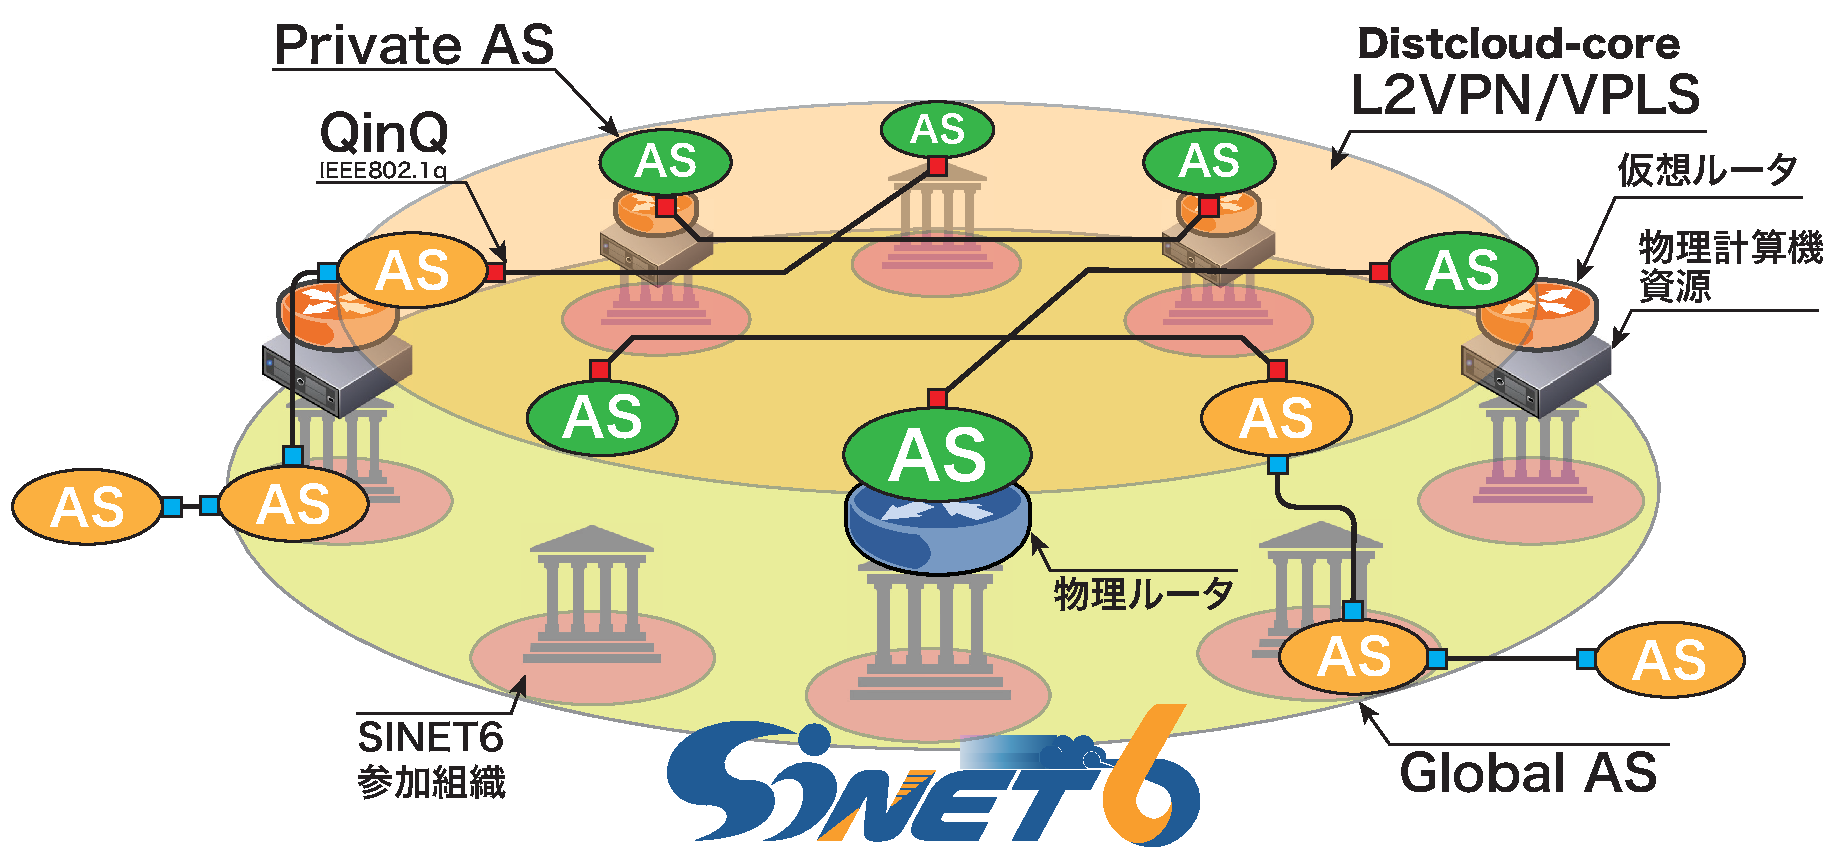
\includegraphics[width=84mm,clip]{AS_dojo.pdf}
\caption{提案するEGP演習テストベッド''AS DOJO''の模式図}
\label{AS_dojo}
\end{center}
\end{figure}

\begin{acknowledgment}
この研究は2025年度国立情報学研究所公募型共同研究(251S1-22822)の助成を受けています。
\end{acknowledgment}

\section*{}

\end{document}
